\textbf{Цель работы:}\indent
1) измерение давления насыщенного пара жидкости при разной температуре;\\\indent 
2) вычисление по полученным данным теплоты испарения с помощью уравнения 
Клайперона-Клаузиуса. \\\indent 

\section*{Теоретические сведения}
Теплоту парообразования вычислим по формуле Клайперона-Клазиуса:
\begin{equation}
    \frac{dP}{dT} = \frac{L}{T(V_2 - V_1)}
\end{equation}
где $V_2 = V$ - объем пара, $V_1$ - объем жидкости.\\\indent
Запишем уравнение Ван-дер-Ваальса для насыщенного пара:
\begin{equation}
    \left ( P + \frac{a}{V^2}\right )(V - b)
\end{equation}
С учетом того, что $b$ и $a$ вносят небольшую погрешность, 
при данных давлениях и температурах можно записать:
\begin{equation}
    V = \frac{RT}{P}
\end{equation}
Однако с учетом того, что $V_1 \ll V_2$ получаем:
\begin{equation}
    L = \frac{RT^2}{P}\frac{dP}{dT} = -R\frac{d(\ln P)}{d(1/T)}
\end{equation}

\section*{Экспериментальная установка}
Экспериментальная установка показана на рисунке ниже. В приборе 13 находится 
исследумая жидкость 14. Давление насыщенных паров определятеся по 
ртутному манометру 15. 
\begin{figure}[h!]
    \centering
    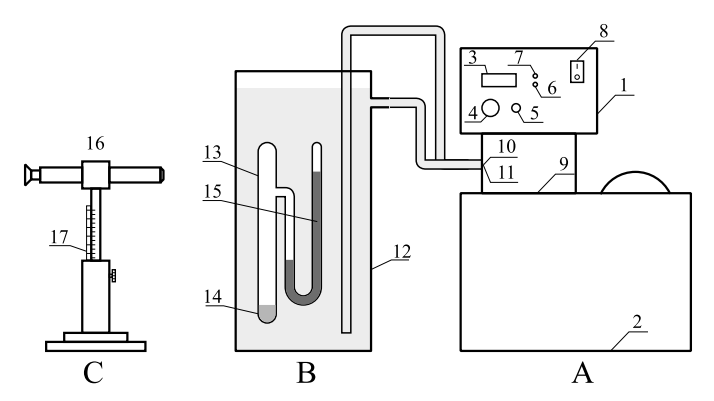
\includegraphics[width=10cm,height=6cm]{setup.png}
    \caption{Схема установки для поределения теплоты испарения}
    \label{fig:setup}
\end{figure}



